% Chapter Template

\chapter{Background} % Main chapter title

\label{Chapter2} % Change X to a consecutive number; for referencing this chapter elsewhere, use \ref{ChapterX}

%----------------------------------------------------------------------------------------
%	SECTION 1
%----------------------------------------------------------------------------------------

Before digging into my specific project, I provide background information that will help to understand my problem domain. Here, I present information on three different topics: the first provides information on the big data software infrastructure that I use in my work; this infrastructure was developed by Project EPIC \parencite{icse11,oopsla12,hiccs15} to support research into an area known as \textit{crisis informatics} \parencite{palen2009,palen2010}. I also present more information on container-orchestration technologies and then discuss microservice architectures in more depth.

\section{Project EPIC}

Project EPIC (Empowering the Public with Information in Crisis) is a project at the University of Colorado Boulder. It conducts research on crisis informatics, an area of study that examines how members of the public make use of social media during times of mass emergency to make sense of a crisis event as well as to coordinate/collaborate around the event.

Project EPIC has a long history of performing software engineering research. Since 2009, Project EPIC has been investigating the software architectures, tools, and techniques needed to produce reliable and scalable \textit{data-intensive software systems}, an area known as \textit{big data software engineering} \parencite{Anderson:2015b}. When large amounts of data are being collected, software engineers need to focus on structuring this data so it is easy to perform analysis and they must work to ensure that this data is easily accessible to analysts. Project EPIC’s big data software engineering research has explored these issues in depth during the creation of the Project EPIC software infrastructure that consists of two major components: EPIC Collect and EPIC Analyze.

EPIC Collect is a 24/7 data collection system that connects to the Twitter Streaming API to collect tweets from various crisis events that need to be monitored in real time. Since 2012, this software has been collecting tweets with an uptime of 99\% and has collected over two billion tweets across hundreds of crisis events. EPIC Collect’s storage layer makes use of Cassandra. This NoSQL database is focused on writes and provides high throughput. EPIC Analyze is a web-based system that makes use of a variety of software frameworks (e.g., Hadoop, Solr, and Redis) to provide various analysis and annotation services for analysts on the large data sets being collected by EPIC Collect. In addition, Project EPIC maintains one machine---known as EPIC Analytics---with a large amount of physical memory to allow analysts to run memory-intensive processes over the collected data.

The software architecture of EPIC Collect and EPIC Analyze is shown in Figure~\ref{fig:epicarch}. Note, this is a logical architecture that does not show how these systems are deployed. For instance, Cassandra is deployed on four machines that run separately from the machines that host the EPIC Collect software, Postgres, Redis, and the Ruby-on-Rails code that makes up EPIC Analyze. In all, the existing Project EPIC infrastructure is distributed across seven machines in a single data center maintained at the University of Colorado Boulder.

\begin{figure}
\centering
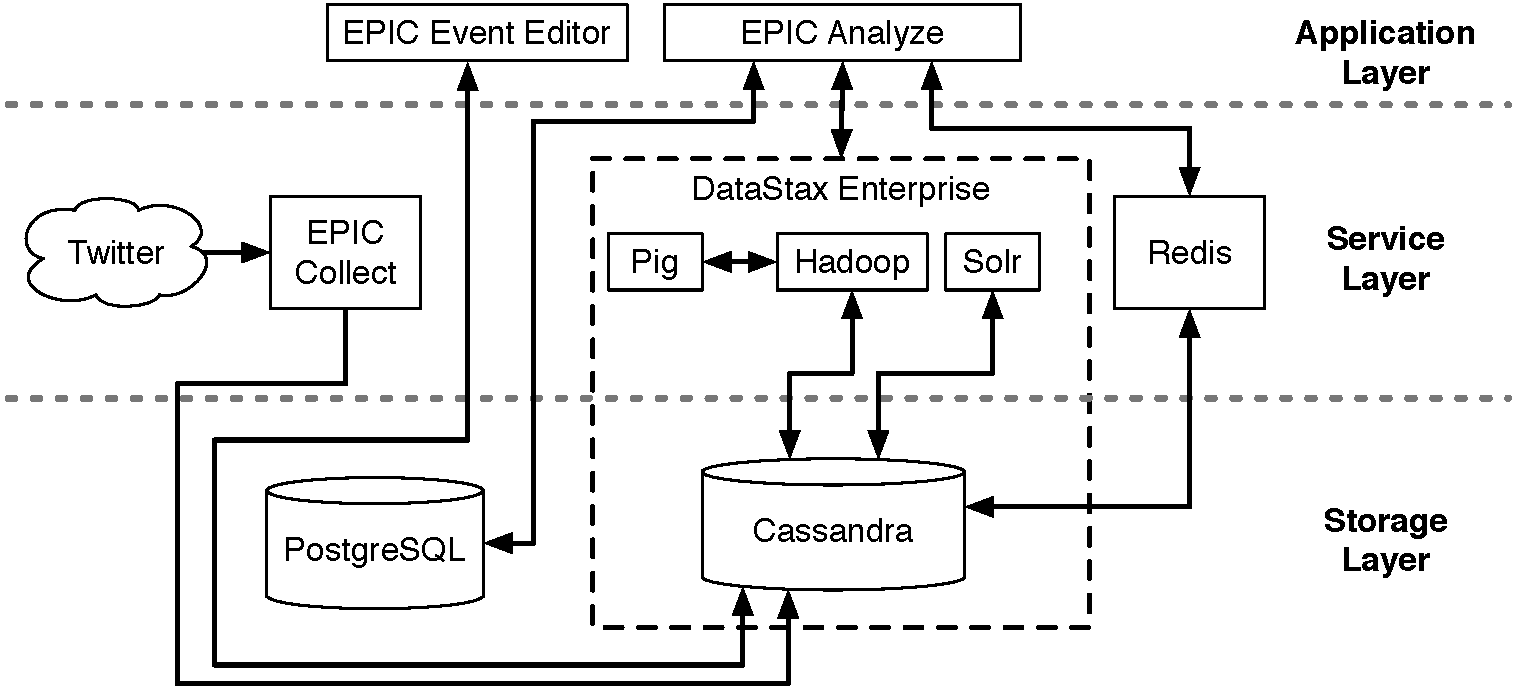
\includegraphics[width=\textwidth]{Figures/old_arch}
\decoRule
\caption[Project EPIC Software Infrastructure]{Project EPIC Software Infrastructure}
\label{fig:epicarch}
\end{figure}


\section{Containerization}

Containerization is a technique that provides operating-system-level virtualization. This technology allows programs to be run inside a \textit{system container}; these containers are isolated from each other as well as from the host machine that is being used to execute them. Containerization works like traditional virtual machines from the point of view of a program, but makes more efficient use of the  system resources on the host machine instead of simulating a full-powered operating system.

There are many containerization platforms available; however, the most widely adopted project is Docker; I will make use of Docker as part of the prototype I built for testing my thesis work. Docker originated as an internal tool for a PaaS (Platform as a Service) company and was later made available as open source. Thanks to many contributions from different companies, this project has grown to become the most used containerization software. It is able to run on almost any machine and many software packages have been made available as Docker containers, providing a wide range of integration opportunities. Finally, almost all existing container orchestration systems support Docker containers.

\section{Container Orchestration Technologies}

As containerization technologies became more widely adopted---spurred by a recent migration to designing systems via microservices---large companies needed a way to manage their containers in a more friendly way. Interconnecting containers, managing their deployment, and scaling them to meet demand, were all possible, but were difficult to achieve. As a result, container orchestration systems were born. To manage containers, these systems add an abstraction layer over containerisation technologies, making such tasks easier to perform.

There are a few container orchestration systems available at the moment. The most popular ones are Kubernetes and Apache Mesos.\footnote{\href{https://kubernetes.io/}{https://kubernetes.io/} and \href{http://mesos.apache.org/}{http://mesos.apache.org/}} In this project, I will make use of Kubernetes. The main reason for this is that---thanks to the open source community---it is easier to find tutorials and courses for Kubernetes. In addition, there are a lot of big companies backing this project and contributing to it; this activity provides evidence that this project will be supported well into the future.

Google Cloud seems like the best fit to host Kubernetes as it has a managed cluster option that makes it straightforward to install and connect system components. In addition, thanks to Google being part of the maintenance team for Kubernetes, there is a great support for the Google Cloud infrastructure within Kubernetes.

\section{Microservices Architecture}

Microservices is an approach to distributed systems that promote the use of small services with specific responsibilities that collaborate between them, rather than making use of big components with a lot of responsibilities that make interaction more difficult. They are thus more cohesive units of software with minimal dependencies between them. A system designed with loosely-coupled, highly-cohesive software components has always been a highly-desirable goal in software design \parencite{gradybook} and microservices help to achieve that goal with distributed software systems.

In addition, thanks to new technologies like containers and container-orchestrated systems, microservices are quickly becoming a standard tool in the design of large software systems. This type of software architecture has been adopted by many companies as it makes maintenance of these systems more straightforward.

Another key advantage of the microservices approach is that it makes it easier to adopt different technologies for each component of your software system. In addition to containerization, it decouples different parts of a system. This separation allows for a better optimization of technology depending on the feature that each microservice needs to provide. For example, a microservice that needs to store highly-related data can make use of a graph database. At the same time, a separate microservice that needs to store and index large documents can use a document store underneath, allowing for a better fit with its needs while allowing both microservices to be deployed as part of a single software system.

Having small microservices do specific tasks makes development cycles faster and more independent. It also makes incremental deployment much easier and less dangerous. Finally, microservices make it easier to scale software systems since one can individually scale parts of the system depending on their usage \parencite{microservicesScale}.

Microservices avoid problems associated with previous approaches to service-oriented architectures by focusing solely on the overall software architecture and letting the architect decide how services are to be deployed or what messaging system is used to communicate between them. In addition, a microservices architecture provides improved reliability and resilience, as each microservice is independent. If one fails, the rest are unaffected. This feature is a perfect match with container-orchestration systems that can easily perform health checks on microservices and redeploy any that have failed.

In terms of designing a microservice architecture, there are two approaches that are equally used at the moment: \textit{choreography} and \textit{orchestration} \parencite{microservices}.


%-----------------------------------
%	SUBSECTION 1
%-----------------------------------
\subsection{Coreography}

Choreography centers all interactions around a publish-subscribe communication model. Events are propagated through the system in an asynchronous manner. When something happens in a microservice, a message gets published on a public queue. Other microservices can subscribe to this queue and respond when they receive that message.

This approach makes a system more flexible, removing the responsibility of knowing how to send messages to other microservices. One can add more components easily without having to modify existing ones. However, we need extra components to make sure that all tasks are performed once an event is published. We can accomplish this by installing and maintaining a monitoring solution.


%-----------------------------------
%	SUBSECTION 2
%-----------------------------------

\subsection{Orchestration}

Orchestration imposes request/response interactions on microservices. Each microservice makes requests directly on other microservices. For this approach to work, one needs a service discovery mechanism. In addition, if a service is down, we need to make sure that microservices are architected to retry failed attempts and to fail gently if a required microservice is unavailable. The benefit to this approach is that, due to the synchronous nature of these interactions, we know that all steps of an activity have been completed when the original call returns. The limitation is that one non-responsive microservice can bring down an entire set of actions.

A more modern approach to orchestration has been developed with service meshes \parencite{servicemesh}. A service mesh has the responsibility of providing service discovery while also balancing requests across multiple instances of a microservice; they also guard against having an activity fail by retrying requests. A service mesh works by adding a sidecar to all microservices allowing it to act as a proxy between a microservice and the outside network. Unfortunately, service meshes are still new technologies that are rapidly evolving; they often lack features found in other approaches such as the extensibility capabilities found in choreography-based systems. As a result, I do not make use of them in my thesis work.

%----------------------------------------------------------------------------------------
%	SECTION 2
%----------------------------------------------------------------------------------------

\section{Messaging systems}

Messaging systems organize queues of messages produced by microservices and notify subscribed components when they arrive. Their main objective is to decouple components and to serve as a cache if consumers cannot process all of the incoming messages. This allows for more reliable systems as a system does not depend on the mutual availability of a sender and a receiver to pass messages as they would if they used other messaging systems, such as HTTP.

There are many options available in this space, with the most popular being Apache Kafka and RabbitMQ. Kafka is a decentralized, high-availability messaging system that allows one to publish messages organized by topics. It allows for high parallelizability thanks to the partitions on topics, which lets one read and write at a higher rate. Each partition can have one consumer associated with it providing faster reads.

Another benefit of Kafka is its persistence system. Thanks to a strong integration with the kernel of the host operating system, it persists data faster than other systems. This is due to the fact that it gives the responsibility of flushing messages to disk to the kernel, taking advantage of optimizations like disk page caching and memory caching implemented in modern operating systems.

In addition, Kafka is one of the most used messaging systems in the industry. Many companies use it in production to decouple their systems. Kafka has a strong community behind it as well, and large organizations (e.g. LinkedIn) take an active role in maintaining it.

Messaging systems are needed for choreography microservice architectures as they serve as the communication layer between microservices.

\section{Big Data Storage Systems}

For my thesis work, I  will be collecting data from Twitter via the Streaming API. This API is limited to provide 1\% of the total tweets generated in Twitter every minute. Based on a report from 2013, I know that rate is approximately 5700 tweets per second on average \parencite{tweetsRecord}. As a result, I can calculate the total number of tweets per second that I estimate will flow through my system prototype per second and that is approximately 57 tweets per second on average as a minimum bound. Since that corresponds to \~4.9M tweets/day, I need a data storage technology that scales to handle large datasets. As previously studied in Project EPIC \parencite{oopsla12}, I need to use a NoSQL database instead of a relational database to support the high volume of tweets that come from this API, making my system more scalable.

On the other hand I also need a system that allows analytical and operational queries to happen at the same time. I would like to be able to analyze my data in real time without having to stop my data collection process. Given that some analysis tasks may take a few minutes due to the high number of tweets, I need to have a system that supports high throughput for both parts (collection and analsyis). In this case, Cassandra is an excellent option as the number of operations it can perform per second scales better compared to other NoSQL alternatives, especially with operational and analytical workloads.\parencite{benchmarkNoSQL}

To store tweets, I base my table structure on the current EPIC Analyze column family structure in Cassandra as described by the CQL code in Listing~\ref{lst:cql}. I have added an index on the event\_name attribute so that I can access events faster. I need this index as many queries are performed per event.

\begin{lstlisting}[language=SQL, caption={Tweets CQL table script}, float, floatplacement=H, label={lst:cql}]
CREATE TABLE twitter_analytics.tweet (
    id uuid,
    t_id text,
    event_kw text,
    event_name text,
    hashtags list<text>,
    media_url text,
    t_coordinates text,
    t_created_at timestamp,
    t_favorite_count int,
    t_favorited boolean,
    t_geo text,
    t_is_a_retweet boolean,
    t_lang text,
    t_retweet_count int,
    t_retweeted boolean,
    t_text text,
    u_created_at timestamp,
    u_description text,
    u_favourites_count int,
    u_followers_count int,
    u_friends_count int,
    u_geo_enabled boolean,
    u_id text,
    u_lang text,
    u_listed_count int,
    u_location text,
    u_name text,
    u_screen_name text,
    u_statuses_count int,
    u_time_zone text,
    u_url text,
    u_utc_offset int,
    um_id text,
    um_name text,
    um_screen_name text,
    urls list<text>,
    PRIMARY KEY (id, t_id))
\end{lstlisting}

